\documentclass[11pt,a4paper,]{article}
\usepackage{lmodern}

\usepackage{amssymb,amsmath}
\usepackage{ifxetex,ifluatex}
\usepackage{fixltx2e} % provides \textsubscript
\ifnum 0\ifxetex 1\fi\ifluatex 1\fi=0 % if pdftex
  \usepackage[T1]{fontenc}
  \usepackage[utf8]{inputenc}
\else % if luatex or xelatex
  \usepackage{unicode-math}
  \defaultfontfeatures{Ligatures=TeX,Scale=MatchLowercase}
\fi
% use upquote if available, for straight quotes in verbatim environments
\IfFileExists{upquote.sty}{\usepackage{upquote}}{}
% use microtype if available
\IfFileExists{microtype.sty}{%
\usepackage[]{microtype}
\UseMicrotypeSet[protrusion]{basicmath} % disable protrusion for tt fonts
}{}
\PassOptionsToPackage{hyphens}{url} % url is loaded by hyperref
\usepackage[unicode=true]{hyperref}
\hypersetup{
            pdftitle={ETC513 Assignment 3: Comparison of Energy and Pollution by Country},
            pdfborder={0 0 0},
            breaklinks=true}
\urlstyle{same}  % don't use monospace font for urls
\usepackage{geometry}
\geometry{a4paper, centering, text={16cm,24cm}}
\usepackage[style=authoryear-comp,]{biblatex}
\addbibresource{references.bib}
\usepackage{longtable,booktabs}
% Fix footnotes in tables (requires footnote package)
\IfFileExists{footnote.sty}{\usepackage{footnote}\makesavenoteenv{long table}}{}
\usepackage{graphicx,grffile}
\makeatletter
\def\maxwidth{\ifdim\Gin@nat@width>\linewidth\linewidth\else\Gin@nat@width\fi}
\def\maxheight{\ifdim\Gin@nat@height>\textheight\textheight\else\Gin@nat@height\fi}
\makeatother
% Scale images if necessary, so that they will not overflow the page
% margins by default, and it is still possible to overwrite the defaults
% using explicit options in \includegraphics[width, height, ...]{}
\setkeys{Gin}{width=\maxwidth,height=\maxheight,keepaspectratio}
\IfFileExists{parskip.sty}{%
\usepackage{parskip}
}{% else
\setlength{\parindent}{0pt}
\setlength{\parskip}{6pt plus 2pt minus 1pt}
}
\setlength{\emergencystretch}{3em}  % prevent overfull lines
\providecommand{\tightlist}{%
  \setlength{\itemsep}{0pt}\setlength{\parskip}{0pt}}
\setcounter{secnumdepth}{5}

% set default figure placement to htbp
\makeatletter
\def\fps@figure{htbp}
\makeatother


\title{ETC513 Assignment 3: Comparison of Energy and Pollution by Country}

%% MONASH STUFF

%% CAPTIONS
\RequirePackage{caption}
\DeclareCaptionStyle{italic}[justification=centering]
 {labelfont={bf},textfont={it},labelsep=colon}
\captionsetup[figure]{style=italic,format=hang,singlelinecheck=true}
\captionsetup[table]{style=italic,format=hang,singlelinecheck=true}


%% FONT
\RequirePackage{bera}
\RequirePackage[charter,expert,sfscaled]{mathdesign}
\RequirePackage{fontawesome}

%% HEADERS AND FOOTERS
\RequirePackage{fancyhdr}
\pagestyle{fancy}
\rfoot{\Large\sffamily\raisebox{-0.1cm}{\textbf{\thepage}}}
\makeatletter
\lhead{\textsf{\expandafter{\@title}}}
\makeatother
\rhead{}
\cfoot{}
\setlength{\headheight}{15pt}
\renewcommand{\headrulewidth}{0.4pt}
\renewcommand{\footrulewidth}{0.4pt}
\fancypagestyle{plain}{%
\fancyhf{} % clear all header and footer fields
\fancyfoot[C]{\sffamily\thepage} % except the center
\renewcommand{\headrulewidth}{0pt}
\renewcommand{\footrulewidth}{0pt}}

%% MATHS
\RequirePackage{bm,amsmath}
\allowdisplaybreaks

%% GRAPHICS
\RequirePackage{graphicx}
\setcounter{topnumber}{2}
\setcounter{bottomnumber}{2}
\setcounter{totalnumber}{4}
\renewcommand{\topfraction}{0.85}
\renewcommand{\bottomfraction}{0.85}
\renewcommand{\textfraction}{0.15}
\renewcommand{\floatpagefraction}{0.8}


%\RequirePackage[section]{placeins}

%% SECTION TITLES


%% SECTION TITLES (NEW: Changing sections and subsections color)
\RequirePackage[compact,sf,bf]{titlesec}
\titleformat*{\section}{\Large\sf\bfseries\color[rgb]{0.8, 0.7, 0.1 }}
\titleformat*{\subsection}{\large\sf\bfseries\color[rgb]{0.8, 0.7, 0.1 }}
\titleformat*{\subsubsection}{\sf\bfseries\color[rgb]{0.8, 0.7, 0.1 }}
\titlespacing{\section}{0pt}{2ex}{.5ex}
\titlespacing{\subsection}{0pt}{1.5ex}{0ex}
\titlespacing{\subsubsection}{0pt}{.5ex}{0ex}


%% TITLE PAGE
\def\Date{\number\day}
\def\Month{\ifcase\month\or
 January\or February\or March\or April\or May\or June\or
 July\or August\or September\or October\or November\or December\fi}
\def\Year{\number\year}

%% LINE AND PAGE BREAKING
\sloppy
\clubpenalty = 10000
\widowpenalty = 10000
\brokenpenalty = 10000
\RequirePackage{microtype}

%% PARAGRAPH BREAKS
\setlength{\parskip}{1.4ex}
\setlength{\parindent}{0em}

%% HYPERLINKS
\RequirePackage{xcolor} % Needed for links
\definecolor{darkblue}{rgb}{0,0,.6}
\RequirePackage{url}

\makeatletter
\@ifpackageloaded{hyperref}{}{\RequirePackage{hyperref}}
\makeatother
\hypersetup{
     citecolor=0 0 0,
     breaklinks=true,
     bookmarksopen=true,
     bookmarksnumbered=true,
     linkcolor=darkblue,
     urlcolor=blue,
     citecolor=darkblue,
     colorlinks=true}

\usepackage[showonlyrefs]{mathtools}
\usepackage[no-weekday]{eukdate}

%% BIBLIOGRAPHY

\makeatletter
\@ifpackageloaded{biblatex}{}{\usepackage[style=authoryear-comp, backend=biber, natbib=true]{biblatex}}
\makeatother
\ExecuteBibliographyOptions{bibencoding=utf8,minnames=1,maxnames=3, maxbibnames=99,dashed=false,terseinits=true,giveninits=true,uniquename=false,uniquelist=false,doi=false, isbn=false,url=true,sortcites=false}

\DeclareFieldFormat{url}{\texttt{\url{#1}}}
\DeclareFieldFormat[article]{pages}{#1}
\DeclareFieldFormat[inproceedings]{pages}{\lowercase{pp.}#1}
\DeclareFieldFormat[incollection]{pages}{\lowercase{pp.}#1}
\DeclareFieldFormat[article]{volume}{\mkbibbold{#1}}
\DeclareFieldFormat[article]{number}{\mkbibparens{#1}}
\DeclareFieldFormat[article]{title}{\MakeCapital{#1}}
\DeclareFieldFormat[article]{url}{}
%\DeclareFieldFormat[book]{url}{}
%\DeclareFieldFormat[inbook]{url}{}
%\DeclareFieldFormat[incollection]{url}{}
%\DeclareFieldFormat[inproceedings]{url}{}
\DeclareFieldFormat[inproceedings]{title}{#1}
\DeclareFieldFormat{shorthandwidth}{#1}
%\DeclareFieldFormat{extrayear}{}
% No dot before number of articles
\usepackage{xpatch}
\xpatchbibmacro{volume+number+eid}{\setunit*{\adddot}}{}{}{}
% Remove In: for an article.
\renewbibmacro{in:}{%
  \ifentrytype{article}{}{%
  \printtext{\bibstring{in}\intitlepunct}}}

\AtEveryBibitem{\clearfield{month}}
\AtEveryCitekey{\clearfield{month}}

\makeatletter
\DeclareDelimFormat[cbx@textcite]{nameyeardelim}{\addspace}
\makeatother

\author{\sf\Large\textbf{ Shaohu Chen}\\ {\sf\large Master of Business Analytics(In Progress)\\[0.5cm]} \sf\Large\textbf{ Qian Duan}\\ {\sf\large Master of Business Analytics(In Progress)\\[0.5cm]} \sf\Large\textbf{ Tina Tsou}\\ {\sf\large Master of Business Analytics(In Progress)\\[0.5cm]}}

\date{\sf\Date~\Month~\Year}
\makeatletter
\lfoot{\sf Chen, Duan, Tsou: \@date}
\makeatother


%%%% PAGE STYLE FOR FRONT PAGE OF REPORTS

\makeatletter
\def\organization#1{\gdef\@organization{#1}}
\def\telephone#1{\gdef\@telephone{#1}}
\def\email#1{\gdef\@email{#1}}
\makeatother
  \organization{Australian Government COVID19}

  \def\name{Our consultancy \newline add names \&\newline add names}

  \telephone{(03) 9905 2478}

  \email{questions@company.com}                 %NEW: New email addresss

\def\webaddress{\url{http://company.com/stats/consulting/}} %NEW: URl
\def\abn{12 377 614 630}                                    % NEW: ABN
\def\logo{\includegraphics[width=6cm]{logo}}  %NEW: Changing logo
\def\extraspace{\vspace*{1.6cm}}
\makeatletter
\def\contactdetails{\faicon{phone} & \@telephone \\
                    \faicon{envelope} & \@email}
\makeatother

%%%% FRONT PAGE OF REPORTS

\def\reporttype{Report for}

\long\def\front#1#2#3{
\newpage
\begin{singlespacing}
\thispagestyle{empty}
\vspace*{-1.4cm}
\hspace*{-1.4cm}
\hbox to 16cm{
  \hbox to 6.5cm{\vbox to 14cm{\vbox to 25cm{
    \logo
    \vfill
    \parbox{6.3cm}{\raggedright
      \sf\color[rgb]{0.8, 0.7, 0.1 }    % NEW color 
      {\large\textbf{\name}}\par
      \vspace{.7cm}
      \tabcolsep=0.12cm\sf\small
      \begin{tabular}{@{}ll@{}}\contactdetails
      \end{tabular}
      \vspace*{0.3cm}\par
      ABN: \abn\par
    }
  }\vss}\hss}
  \hspace*{0.2cm}
  \hbox to 1cm{\vbox to 14cm{\rule{4pt}{26.8cm}\vss}\hss\hfill}  %NEW: Thicker line
  \hbox to 10cm{\vbox to 14cm{\vbox to 25cm{   
      \vspace*{3cm}\sf\raggedright
      \parbox{11cm}{\sf\raggedright\baselineskip=1.2cm
         \fontsize{24.88}{30}\color[rgb]{0, 0.29, 0.55}\sf\textbf{#1}}   % NEW: title color blue
      \par
      \vfill
      \large
      \vbox{\parskip=0.8cm #2}\par
      \vspace*{2cm}\par
      \reporttype\\[0.3cm]
      \hbox{#3}%\\[2cm]\
      \vspace*{1cm}
      {\large\sf\textbf{\Date~\Month~\Year}}
   }\vss}
  }}
\end{singlespacing}
\newpage
}

\makeatletter
\def\titlepage{\front{\expandafter{\@title}}{\@author}{\@organization}}
\makeatother

\usepackage{setspace}
\setstretch{1.5}

%% Any special functions or other packages can be loaded here.
\usepackage{booktabs}
\usepackage{longtable}
\usepackage{array}
\usepackage{multirow}
\usepackage{wrapfig}
\usepackage{float}
\usepackage{colortbl}
\usepackage{pdflscape}
\usepackage{tabu}
\usepackage{threeparttable}
\usepackage{threeparttablex}
\usepackage[normalem]{ulem}
\usepackage{makecell}
\usepackage{xcolor}


\begin{document}
\titlepage

\section*{Introduction}

\begin{itemize}
\tightlist
\item
  Data Description:
\end{itemize}

This data set is \href{https://data.gov.au/dataset/ds-qld-3f90a4c3-23df-49dc-b243-9a29c0b23dd5/details?q=Practical\%20driving}{Practical driving examination results for customers} which is provided by local government authority (LGA) of Queensland. It records the license class, booking type, examination results and driver age group during 2005 to 2019.

\begin{itemize}
\tightlist
\item
  Research aims:
\end{itemize}

We divided into three parts, the first part focuses on the annual pass rate of different local government authority.

The second part mainly aims to compare the age group with different license.

The third part calculates the correlation between the examination results and booking type.

\section*{Step 1}

The first part focuses on the annual pass rate of different local government authority.

\begin{figure}
\centering
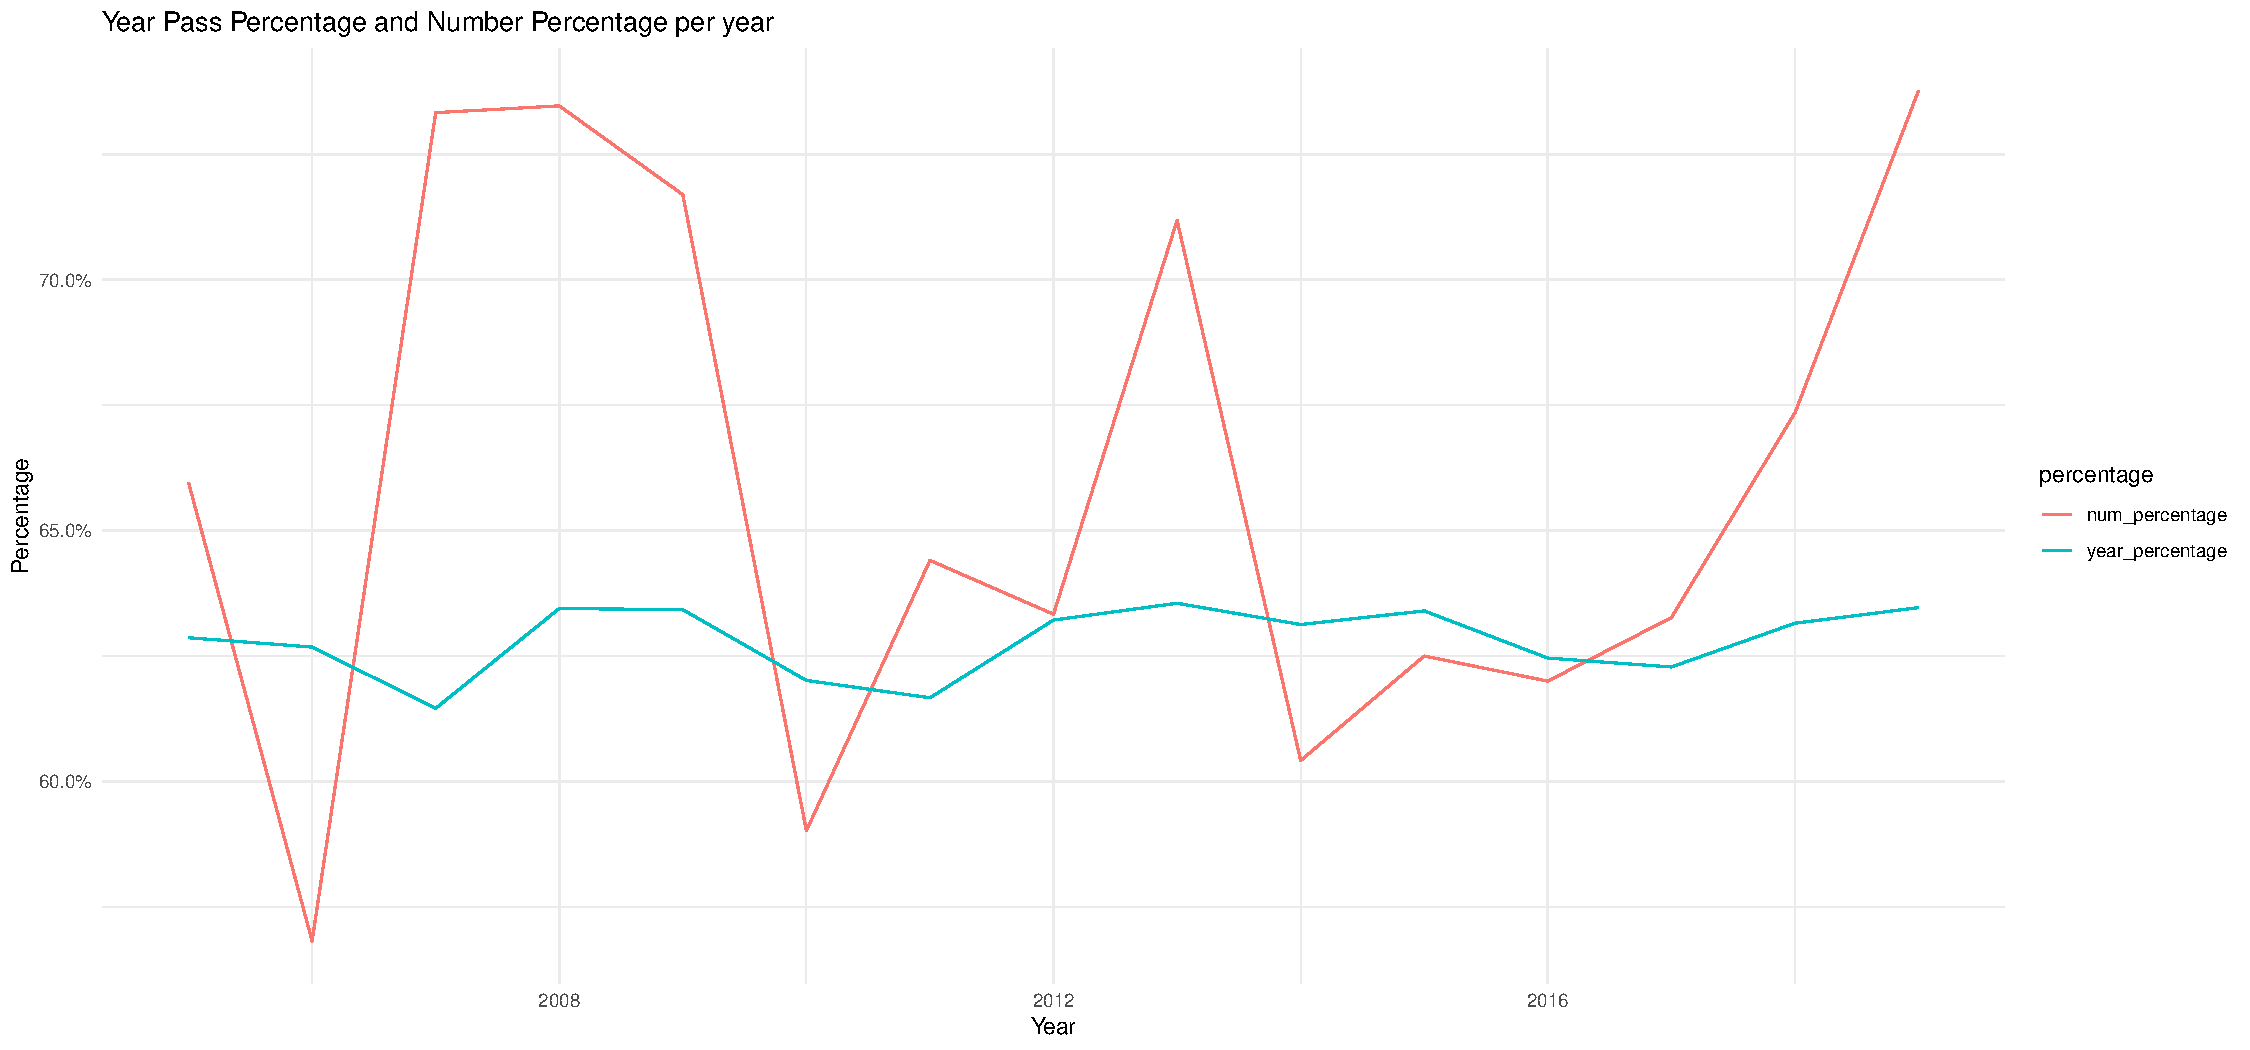
\includegraphics{Assignment4_files/figure-latex/Fig1-1.pdf}
\caption{\label{fig:Fig1}Year Pass Percentage(year\_percentage) and Percentage of Local Government Authority annual passing rates exceeding the total annual passing rate(num\_percentage)}
\end{figure}

In the figure \ref{fig:Fig1}, as for the annual pass rate, it does not fluctuate greatly, and basically remained at 62.5\% but the percentage of the number exceeding the annual pass rate fluctuates greatly, which may be due to missing data in some regions, however, from the data point of view, it has been in an upward phase in recent years.

\begin{table}

\caption{\label{tab:Tab1}Number of time getteing the highest pass rate per year}
\centering
\begin{tabular}[t]{lr}
\toprule
Local Government Authority & count\\
\midrule
BLACKALL-TAMBO REGIONAL COUNCIL & 5\\
BALONNE SHIRE COUNCIL & 4\\
HOPE VALE ABORIGINAL SHIRE COUNCIL & 4\\
MOBILE SERVICES & 4\\
BARCALDINE REGIONAL COUNCIL & 3\\
\addlinespace
BURKE SHIRE COUNCIL & 3\\
\bottomrule
\end{tabular}
\end{table}

\begin{table}

\caption{\label{tab:Tab2}Number of time getteing the lowest pass rate per year}
\centering
\begin{tabular}[t]{lr}
\toprule
Local Government Authority & count\\
\midrule
MAREEBA SHIRE COUNCIL & 2\\
NAPRANUM ABORIGINAL SHIRE COUNCIL & 2\\
REDLAND CITY COUNCIL & 2\\
BURDEKIN SHIRE COUNCIL & 1\\
HOPE VALE ABORIGINAL SHIRE COUNCIL & 1\\
\addlinespace
KOWANYAMA ABORIGINAL SHIRE CONUNCIL & 1\\
\bottomrule
\end{tabular}
\end{table}

In the table \ref{tab:Tab1}, BLACKALL-TAMBO REGIONAL COUNCIL has the most number of first (5 times). In the table \ref{tab:Tab2}, MAREEBA SHIRE COUNCIL, NAPRANUM ABORIGINAL SHIRE COUNCIL, REDLAND CITY COUNCIL have won the last 2 times.

\begin{figure}
\centering
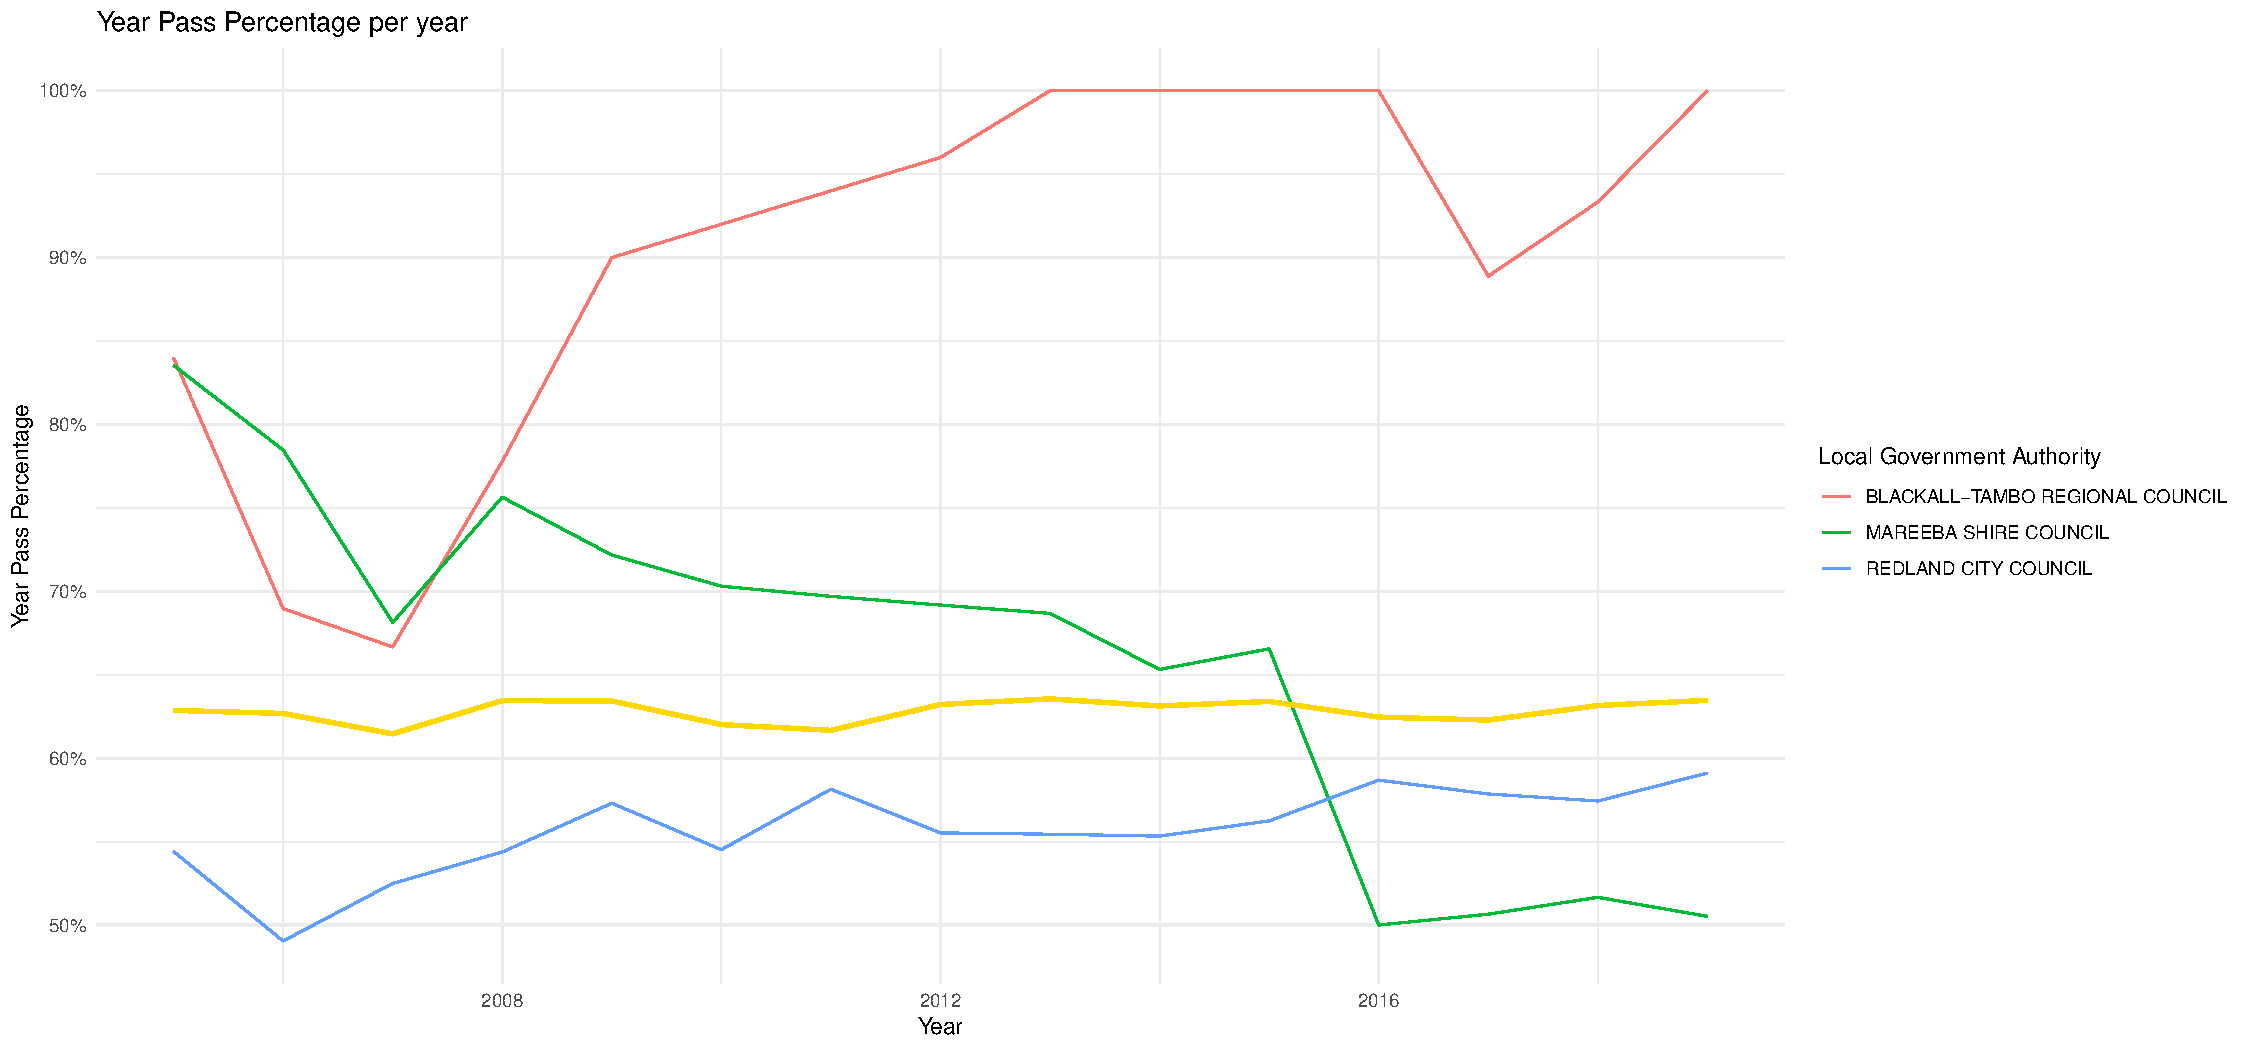
\includegraphics{Assignment4_files/figure-latex/Fig2-1.pdf}
\caption{\label{fig:Fig2}Year Pass Percentage in BLACKALL-TAMBO REGIONAL COUNCIL, BLACKALL-TAMBO REGIONAL COUNCIL, and REDLAND CITY COUNCIL}
\end{figure}

According to the figure \ref{fig:Fig2}, the annual pass rate of BLACKALL-TAMBO REGIONAL COUNCIL has been on the rise after 2007, even reaching 100\%, while the annual pass rate of MAREEBA SHIRE COUNCIL is in a downward state, and the annual pass rate of REDLAND CITY COUNCIL basically fluctuates at 55\%. Especially, MAREEBA SHIRE COUNCIL and REDLAND CITY COUNCIL have been lower than the annual pass rate since 2015, which the gold line is year pass rate.

\begin{figure}
\centering
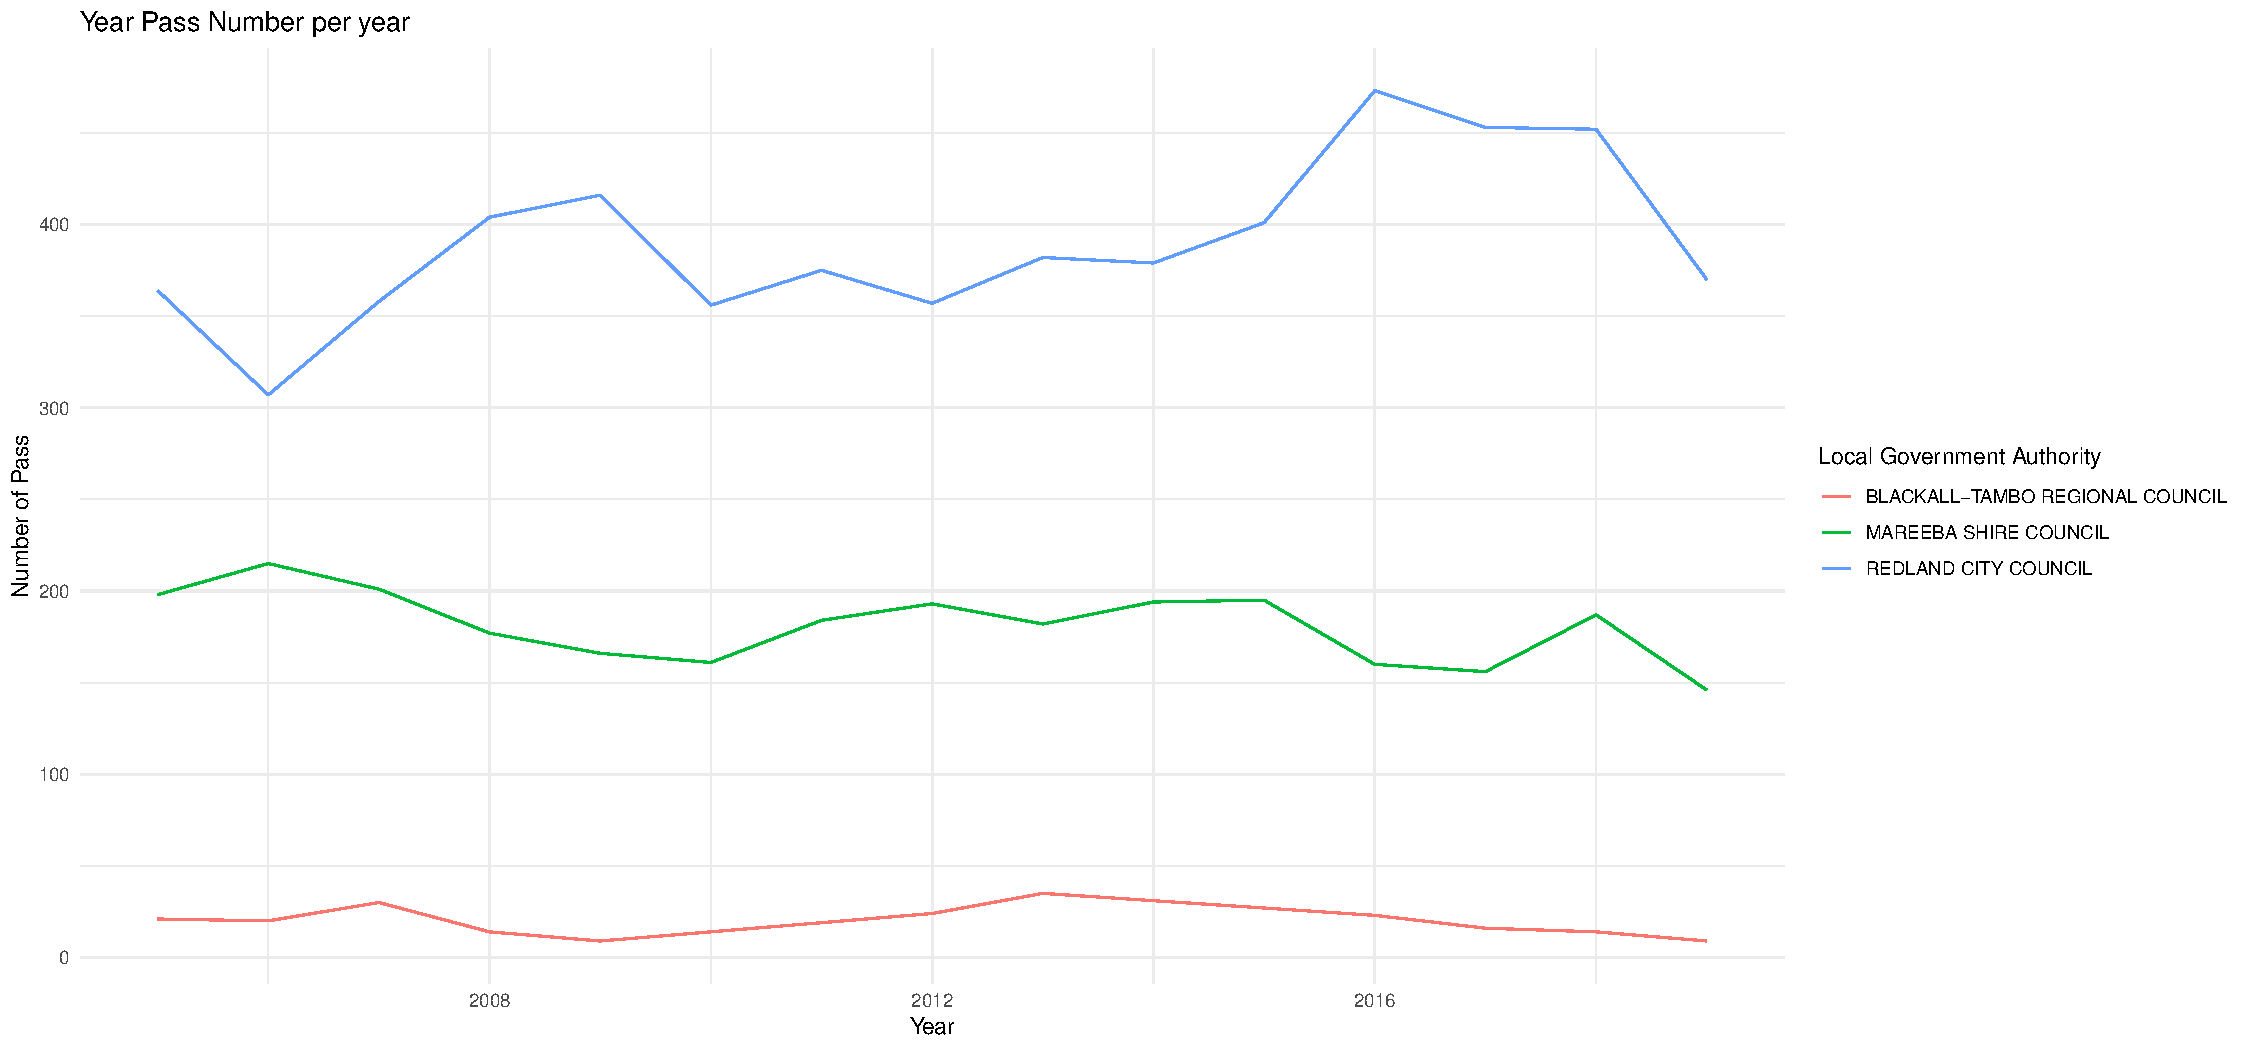
\includegraphics{Assignment4_files/figure-latex/Fig3-1.pdf}
\caption{\label{fig:Fig3}Year Pass Number in BLACKALL-TAMBO REGIONAL COUNCIL, MAREEBA SHIRE COUNCIL, and REDLAND CITY COUNCIL}
\end{figure}

In the figure \ref{fig:Fig3}, the number of pass for three government authorities basically has little fluctuation. Interestingly, the ranking of the number of passes and the ranking of the pass rate are completely opposite.

Therefore, the annual pass rate has not changed much, the percentage of the number exceeding the annual pass rate fluctuates greatly. Areas with sparsely populated areas may have fewer people participating, resulting in a higher overall pass rate than areas with densely populated areas.

\section*{Step 2}

The driving examination pass rate of Queensland is 63\% .

\begin{table}[!h]

\caption{\label{tab:passrate}The pass rate of each product type}
\centering
\begin{tabular}[t]{ll}
\toprule
Product Type Name & pass\_rate\\
\midrule
\cellcolor{gray!6}{CLASS CA - CAR (AUTOMATIC)} & \cellcolor{gray!6}{53\%}\\
CLASS C - CAR (MANUAL) & 56\%\\
\cellcolor{gray!6}{CLASS HR - HEAVY RIGID VEHICLE} & \cellcolor{gray!6}{70\%}\\
CLASS MR - MEDIUM RIGID VEHICLE & 77\%\\
\cellcolor{gray!6}{CLASS RE - MOTORCYCLE (UP TO 250CC} & \cellcolor{gray!6}{77\%}\\
\addlinespace
CLASS HC - HEAVY COMBINATION VEHICLE & 79\%\\
\cellcolor{gray!6}{CLASS LR - LIGHT RIGID VEHICLE} & \cellcolor{gray!6}{83\%}\\
CLASS R - MOTORCYCLE (OVER 250CC) & 86\%\\
\bottomrule
\end{tabular}
\end{table}

\begin{itemize}
\item
  The table \ref{tab:passrate} is the pass rate of different licenses. Above all, the automatic car has the lowest passing rate with 53\%, Since the car has the largest amount of popularity to meet people daily command, so there are more people to join the test of cars.
\item
  While the motorcycle over 250cc has the largest pass rate with 86\%. The motorcycle is much more professional, and it required people got the license up to 250cc who can take part in the test. Therefore, these people are professional so got a higher rate.
\end{itemize}

\begin{figure}

{\centering 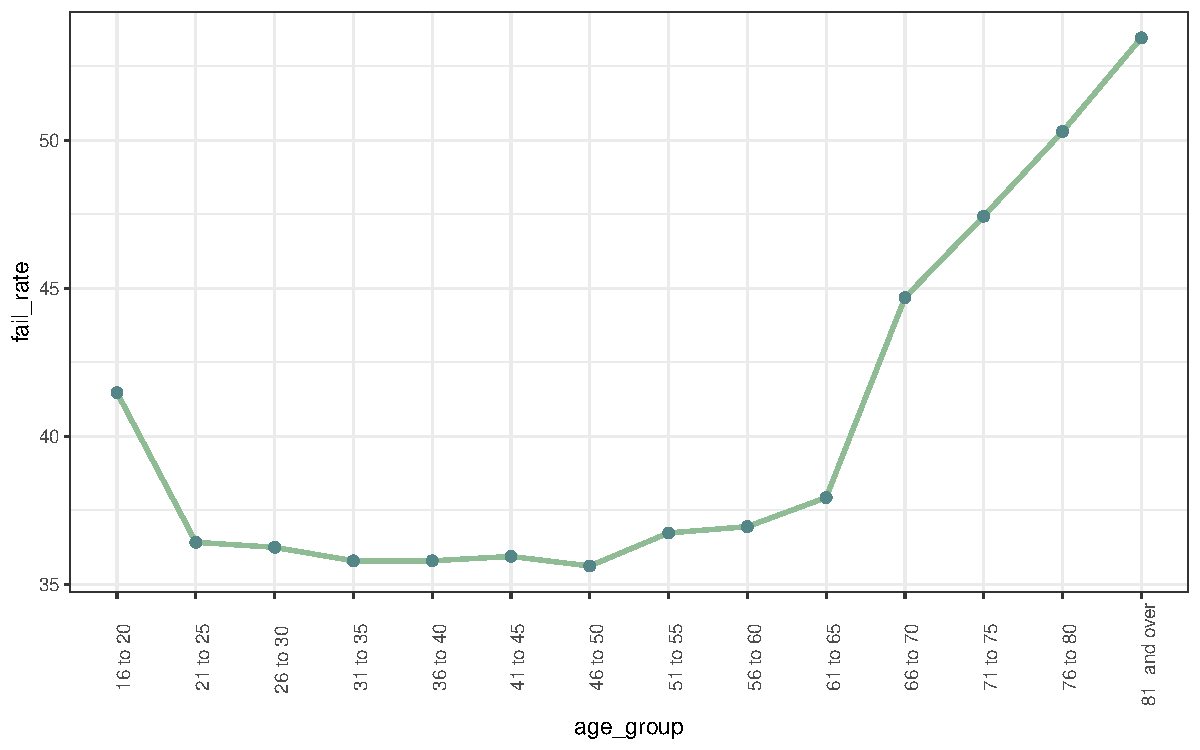
\includegraphics{Assignment4_files/figure-latex/failrate-1} 

}

\caption{Queensland driving test fail rates by age}\label{fig:failrate}
\end{figure}

Figure \ref{fig:failrate}, describes the failing rate of different age groups. It can be seen that the fail rate is increasing with the age grows older. Because people is 81 years old and over has the highest fail rate, which means it is hard for people to pass the driving license after 61 years old. However, there is one interesting point for young people with high rate at 41\%. Basically, the people in this range takes the highest number of examinations. While in the original data set, some young people around these ages have 200- or 300-times test, but still failed. Australia government has more restrictions on young people driving license, so the rate is high.

\begin{figure}
\centering
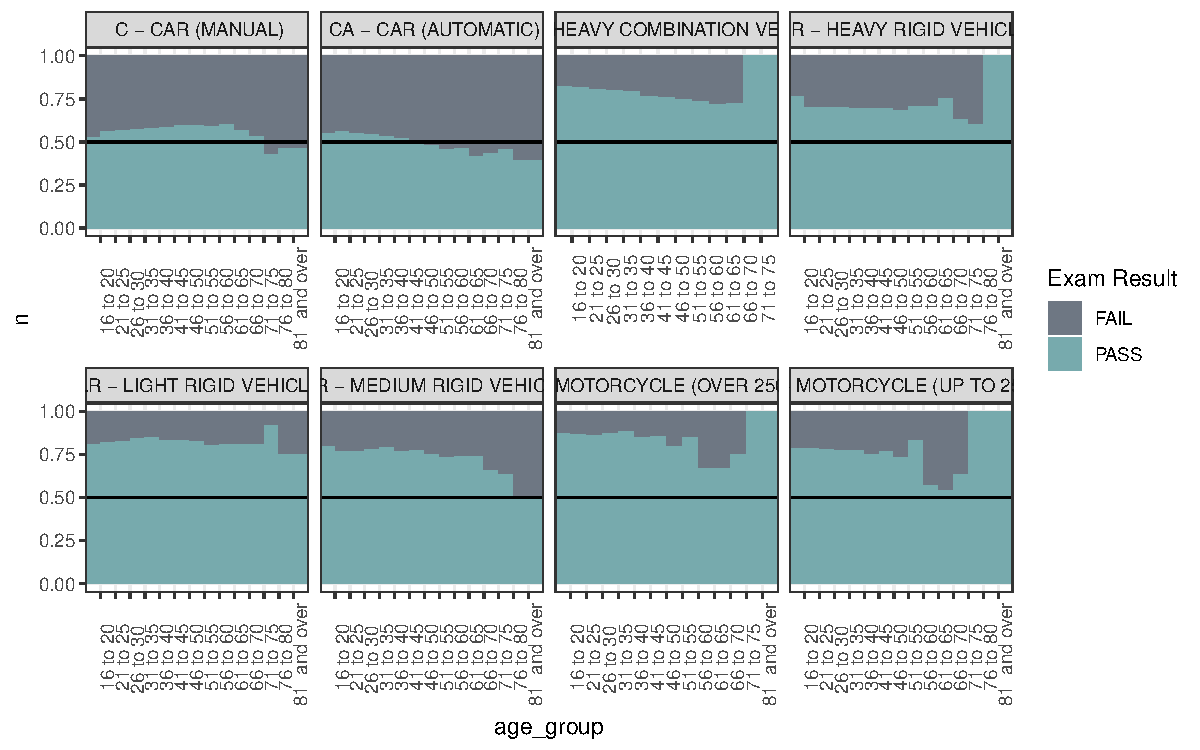
\includegraphics{Assignment4_files/figure-latex/license-1.pdf}
\caption{\label{fig:license}Compare the fail and pass in different license}
\end{figure}

In Figure \ref{fig:license}, for most drive license, the number of pass all exceeds 50\% of all age, except the automatic car license. People who fails at an older age. The number of fails is much more than pass.
Another interesting point is that in motorcycle and heavy vehicle, people over 70 years old get 100\% pass rate. This is mainly because there are only one or two people join the test and he pass. So, the pass rate is 100\%. This doesn't mean all old people can get the license for one time.

\section*{Step 3}

\printbibliography

\end{document}
